% !TeX spellcheck = en_GB
\usetikzlibrary{automata, positioning}



\section*{Mathematical Modelling: Using Markov chains to model bathroom queues}
\vspace{-.30cm}

\title{Mathematical Modelling: Using Markov chains to model bathroom queues}

\begin{center}
	\textbf{Johnny Wong}\footnote{%
		Johnny Wong is a recent graduate of UNSW, Australia ({\tt johnny.c.wong@unswalumni.com})}
\end{center}

\vspace{5mm}

You come home from your morning run sweaty and ready to shower. As you saunter to the bathroom, you see the locked door and bow your head in defeat. Standing in your sweat soaked singlet, your little brother pokes his head out of his room, chucks a deodorant at you before telling you he has dibs on the bathroom after you sister is finished. You throw the deodorant can back at him and curse your house for having so few bathrooms.

Everyone has waited to use the bathroom at some point in their lives. It's common sense that with fewer bathrooms or more people, the longer you'd have to wait. But can we mathematically calculate how long we can expect to wait every day? One approach is with a technique called Markov chains.

For the rest of the article, let's consider a household with 1 bathroom between 4 people.

\subsection*{Markov chains}
To set up a Markov chain, you need several things: \textbf{states} that represent the possible scenarios, \textbf{probabilities} of moving from state to state throughout some measure of \textbf{time}. We will unpack these 3 things in more detail below.

\subsubsection*{States}
A state is something that can describe the situation of interest at different points in time.

For our bathroom queueing problem, we are interested in how many people are using, or wanting to use, the bathroom at any point in time. So how many states do we need? Well with 4 people, there can be from 0 to 4 people wanting to use the bathroom, meaning we need 5 states. 

Let's label each state $0, \cdots, 5$, where state 0 means no one is wanting to use the bathroom. State 4 means four people want to use the bathroom, since there is only one bathroom available, this means 1 person is using it and there are 3 queuing up.

\subsubsection*{Time}
Time can be either discrete or continuous. With this scenario, it is most appropriate to use continuous time as people can enter and leave the bathroom at any point in time.

Let's represent the state at time $t$ as $X_t$

\subsubsection*{Probability}
How does the system jump from state to state? A fundamental assumption of Markov chains is that the probability of moving from any state to the next is not impacted by any past information, and only depends on the current state.

In continuous time, these probabilities are represented as transition rates of moving from state to state.

\paragraph{Transition rates}
What is a transition rate? Roughly speaking, it is the probability per time unit that the system makes a transition from one state to the other. 
if $q_{i,j}$ represents the transition rate from state $i$ to state $j$ where $i\neq j$, and if the current state is $i$, the probability that the state is $j$ after time $h$ has passed is roughly $h\times q_{i,j}$ for small $h$:
\begin{align*}
h\times q_{i,j} &\approx Pr(X_{t+h} = j|X_t = i)\\
q_{i, j} &\approx \frac{Pr(X_{t+h} = j|X_t = i)}{h} \qquad \text{for small } h
\end{align*}


More precisely,
$$ q_{i,j} = \lim_{h\rightarrow0}\frac{Pr(X_{t+h} = j | X_t = i)}{h} $$

\begin{comment}
	As you can imagine, the transition rate affects the expected time until the there is a transition. If the transition rate out of a state is $\lambda$, then the expected time until a transition is $\frac{1}{\lambda}$ time units.
\\
\end{comment}

Of course, when we specify rates, we need to specify a standard unit of time. It doesn't matter what we choose, but let's express rates as per minute. 

So if $q_{0, 1} = 0.2$, then there is a roughly 20\% chance that if the system is currently in state 0, it will be in state 1 after one minute.

\paragraph{Determining transition rates}
Let's consider a house of just one person. If the person is not currently in the bathroom, what is the transition rate of them going to the bathroom? A quick Google search suggests that people go to the toilet around 7 times a day. Taking into account time spent sleeping (approximated at 8 hours), that's a rate of 7 times per 16 hours, or $\frac{7}{(16 \times 60)} = 0.0073$ per minute. Denote this as $\lambda$.

Bathroom trips take a varying amount of time. For simplicity, let's assume an average trip takes 5 minutes. This implies a certain transition rate of leaving the bathroom. In Markov chain models, the transition rate out of a state is the inverse of the expected time spent in the state. If we let this transition rate be denoted by $\mu$, then $\mu = \frac{1}{5} = 0.2 $
\\

Now that we have estimates for $\lambda$, the rate of one person going to the bathroom, and $\mu$, the rate of one person leaving the bathroom, we can easily determine the transition rate between states. 

\begin{figure}[H]
	\centering
	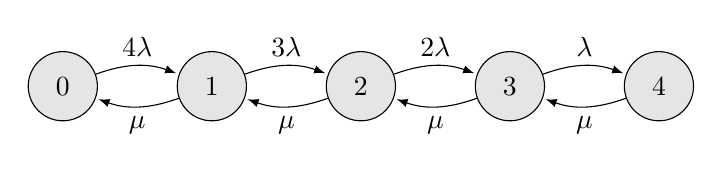
\begin{tikzpicture}
	% Setup the style for the states
	\tikzset{node style/.style={state, 
			fill=gray!20!white}}
	
	\node[node style]               (0)   {0};
	\node[node style, right=of 0]   (1)  {1};
	\node[node style, right=of 1]  (2) {2};
	\node[node style, right=of 2] (3)  {3};
	\node[node style, right=of 3]  (4)   {4};
	
	\draw[>=latex,
	auto=left,
	every loop]
	(0)   edge[bend left=20] node {$4\lambda$}     	(1)
	(1)   edge[bend left=20] node {$\mu$}     		(0)
	(1)   edge[bend left=20] node {$3\lambda$}     (2)
	(2)   edge[bend left=20] node {$\mu$}     (1)
	(2)   edge[bend left=20] node {$2\lambda$}     (3)
	(3)   edge[bend left=20] node {$\mu$}     (2)
	(3)   edge[bend left=20] node {$\lambda$}     (4)
	(4)   edge[bend left=20] node {$\mu$}     (3);
	
	\end{tikzpicture}
	\caption{Diagram showing transition rates between the 5 states.}
	\label{fig: bathroom visual}
\end{figure}

In state 0, there are 4 people that can potentially need to use the bathroom, each with a transition rate of $\lambda$, meaning $q_{0, 1} = 4\lambda$. In state 1, there are only 3 people left with the potential to add to the queue, so $q_{1, 2} = 3\lambda$

Using similar logic, we get the general expression:
$$q_{i, i+1} = (4-i)\lambda \qquad \text{for } i < 4 $$

What about the transition rates of leaving the bathroom? In any state apart from 0, one person is using the bathroom, and the rate of transition for that person is $\mu$, leaving us with 
$$q_{i, i-1}=\mu \qquad \text{for } i > 0$$

It is assumed that multiple people can't suddenly need to use the bathroom or leave the bathroom at the exact same time, so each state can only reach the state one above or below it, meaning:
$$q_{i, j} = 0 \qquad \text{for } \abs{i-j}>1 $$

$q_{i, i}$ represents the rate at which the state remains unchanged. This is the same as saying that the state does not transition to any other state, so it is the negative of the sum of all transition rates out of the state:
$$q_{i, i} = -\sum_{j \neq i} q_{i, j} $$

\paragraph{Transition rate matrix}
Once these transition rates have been determined, they can be arranged in matrix form. Each column and row represent a state, and each element of the matrix is the transition rate of moving from the state represented by the row, to the state represented by the column.
$$
Q=
\bordermatrix{	\text{State} 	&\text{0} 	&\text{1}	& \text{2} 	& \text{3} 	& \text{4} \cr
\text{0} 	& -4\lambda &	4\lambda	&	0 			& 0 			& 0	\cr
\text{1} 	&   \mu  	&-(\mu+3\lambda)&3\lambda 		& 0 			& 0	\cr
\text{2} 	&   0  		&	\mu			&-(\mu+2\lambda)&2\lambda 		& 0	\cr
\text{3} 	&   0  		&	0			&	\mu 		&-(\mu+\lambda)	& \lambda\cr
\text{4}	&	0		&	0			&	0			& \mu 			& -\mu}
$$
And after substituting $\mu = 0.2 $ and $\lambda = \frac{7}{(16 \times 60)} $, we get
$$ Q=
\begin{pmatrix}
-0.029	&	0.029	&	0 		& 0 		& 0	\\
0.2  	&	-0.222	& 0.022 	& 0 		& 0	\\
0  		&	0.2		&-0.215		&0.015 		& 0	\\
0  		&	0		&	0.2 	&-0.207		& 0.007\\
0		&	0		&	0		& 0.2 		& -0.2
\end{pmatrix}
$$
You can verify a few things about this transition matrix:
\begin{itemize}
	\item The sum of each row equals 0. This is because the ``rate" at which the state stays the same is exactly negative of the sum of the rates at which the state changes.
	\item The only negative elements are on the diagonal. These represents the rate at which the state are unchanged.
\end{itemize}


\subsubsection*{Long run proportions}
Now that the system is fully described, we can link it to our original problem. Living in a house of 4 people with 1 bathroom, what is the amount of time one could expect to wait for the bathroom each day? The states where someone is waiting to use the bathroom are states 2, 3 and 4, so let's start by calculating the proportion of time we expect this system to be in these states. To do this, we need to find the \textbf{long run proportions} of each state.

Let $\pi_i$ represent the proportion of time the system is spend in state $i$ if run forever. Since these are proportions, we have $\sum\pi_i = 1$

In the long run, the system will reach an equilibrium where everything balances perfectly. In this context, balance can be represented as:
$$ \pi_i  \times -q_{i, i} = \sum_{j \neq i} \pi_j \times q_{j, i} $$

On the left hand side, we have the rate of transition OUT of state $ i $. On the right, we have the rate of transition INTO state $ i $. Equating these imply we have reached the equilibrium.

Another way of writing this is
$$ 0 = \pi_i  \times q_{i, i} + \sum_{i \neq j} \pi_j \times q_{j, i} \qquad \text{for all  }i$$
Now let's define the vectors $\boldsymbol{\pi}= (\pi_0, \cdots, \pi_4)$ and $\mathbf{0}= (0, \cdots, 0)$. Another way to write the above equations is as a homogenous system of linear equations:
$$ \boldsymbol{\pi}Q = \mathbf{0}$$
Where we have the constraint $ \sum\pi_i = 1 $, which can also be expressed as $$\boldsymbol{\pi} E = \mathbf{1} $$
Where $E$ is a 5 by 5 matrix whose elements are all 1, 
$E = \begin{pmatrix}
1		&	\dots	& 1\\
\vdots	&	\ddots	& \vdots\\
1		&	\dots	& 1

\end{pmatrix}
$ and $\mathbf{1} $ is a row vector of 1s.\\

$\boldsymbol{\pi}$ can then be solved:
\begin{align*}
	 \boldsymbol{\pi}Q &= \mathbf{0}\\
	 \boldsymbol{\pi} E &= \mathbf{1}\\
	 \boldsymbol{\pi} (Q + E) &= \mathbf{1}\\
	 \boldsymbol{\pi} & =  \mathbf{1}(Q+E)^{-1}
\end{align*}
Computer packages can be used to solve
\begin{align*}
	(Q+E)^{-1} = \begin{pmatrix}
	0.971	&	1.029	&	1 		& 1 		& 1	\\
	1.2  	&	0.778	& 1.022 	& 1 		& 1	\\
	1  		&	1.2		&0.785		&1.015 		& 1	\\
	1  		&	1		&	1.2 	&0.793		& 1.007\\
	1		&	1		&	1		& 1.2 		& 0.8
	\end{pmatrix}^{-1}
\end{align*}
To get us to our answer:
$$ \boldsymbol{\pi} = ( 8.599\times 10^{-1}, 1.254\times 10^{-1}, 1.372\times 10^{-2}, 1.000\times 10^{-3}, 3.646\times 10^{-5}) $$
Meaning that 86 \% of the time, the bathrooms is empty, and 12.5 \% of the time, there is one person using a bathroom and no one waiting. You can verify that these proportions add up to to 1 (error coming from rounding).

From this, we can sum $\pi_2 + \pi_3 + \pi_4$ to see that $1.48\%$ of the time, there is at least one person waiting to use the bathroom. Out of our 16 waking hours, this corresponds to about 14 minutes a day where at least one person is waiting to use the bathroom.

To find out the amount of time per person, it might be tempting to simply divide that number by 4, but it's not quite so simple. To demonstrate why, consider two people waiting. You start waiting at 12:00, and manage to go at 12:15, your brother starts waiting as 12:05 and manages to go at 12:20. You've each waited 15 minutes, but the total amount of minutes any person was waiting in the house is only 20 minutes. Although you were both waiting from 12:05 to 12:15, this measure doesn't double up the wait time.

You must calculate the sum of everyone's wait time and divide it by the number of people. In the above example, 2 people waited 15 minutes each, so the calculation would be (15 + 15)/2.
\\

To find the sum of everyone's waiting time, notice that 1.372\% of the time, there is one person waiting, 0.1\% of the time, 2 people are waiting, and 0.003646\% of the time, 3 people are waiting. In other words, to get the sum of everyone's waiting time, we do
$$ (1.372\% \times 1 + 0.1\% \times 2 + 0.003646\% \times 3) \times 16 \times 60 \div 4 = 3.8 $$
Leaving each housemate with an expected 3.8 minutes (3 minutes 48 seconds) of waiting time per day.

\subsection*{Waiting time under different scenarios}
The beauty of having a mathematical model is that it can shed insight into the system under different conditions. The calculation above assumed 4 people and 1 bathroom, let's see what the waiting time would be with different numbers of people and bathrooms.

\begin{figure}[H]
	\centering
	\includegraphics[scale=1]{../../images/comparison}
	\caption{Comparing the average waiting time for each person under different scenarios}
	\label{fig: comparison}
\end{figure}

What's interesting to see is that an additional person doesn't add too much to the expected daily waiting time, and adding an extra bathroom dramatically reduces the expected waiting time. Under this model, 3 people sharing one bathroom spend more waiting time than 15 people with 2 bathrooms!

\subsection*{Limitations of the model}
Now that we've answered our original question, it is important to look back on the process and acknowledge any limitations. There are a few key assumptions that are characteristic of Markov chains.

\paragraph{Memorylessness}
One of the main assumptions of Markov chains is the Markov property. This is also referred to as \textit{memorylessness} because it doesn't matter what's happened in the past, the behaviour of the system only depends on what the current state is. 

We've assumed that the expected time spent in the bathroom is 5 minutes. So as soon as someone walks into the bathroom, it is expected they'll leave after 5 minutes. Under the Markov property, if 3 minutes passes and they're still in the bathroom, the expected time left is not 2 minutes, but still 5 minutes.

Similarly, the rate at which someone goes to the bathroom stays the same regardless of if they've gone 10 times already or haven't gone at all.
\\

While memoryless is not necessarily a realistic assumptions, the final implication is that bathroom times are \textit{exponentially distributed} and the number of bathroom trips per day is \textit{Poisson distributed} and this is quite reasonable.

\paragraph{Independence}
Another assumption of the Markov chain model is independence. This assumption states that the each person acts independently of everyone else, and that the time spent in the bathroom is independent of everything. In real life, this assumption is likely not valid. Here are just a few examples of scenarios where independence isn't satisfied
\begin{itemize}
	\item Most people want to use the bathroom at similar times during the day, such as in the morning after waking up and at night before bed, meaning the rate of using the bathroom is dependent on the time of day
	\item The expected time in the bathroom could be dependent on the time of day as most people shower in the morning or night.
	\item The expected time in the bathroom could be dependent on what people have already done in the bathroom today (e.g. already showered)

\end{itemize}

\subsection*{Concluding remarks}
The problem above is a special case of queuing theory. Markov chains can be used to analyse many other practical problems. To name a few, Google uses them to rank webpages, insurers use them to price safe driver discounts, and biologists use them to model population processes.

As discussed above, Markov chains hold certain assumptions that may not be completely accurate in real life. But in the words of renowned statistician George Box, ``All models are wrong but some are useful". Mathematical modelling is never precise, and it is the art of a mathematician that embraces the imperfection and turns it into something useful.

\newpage
\subsection*{Code}
All calculations were done in Python 3. Below is the code used to calculate the numbers in figure \ref{fig: comparison} and display them as the heatmap.
\inputpython{../../bathroom.py}{1}{57}
